\section[Desenvolvimento do Projeto]{Desenvolvimento do Projeto}

\subsection{Repositório do Código Fonte do Projeto}
O projeto foi organizado em três repositórios, separando a documentação dos
códigos responsáveis pela interface e pela lógica de negócio da aplicação. Essa
estrutura permite manter os artefatos do projeto acessíveis de acordo com sua
finalidade e facilita o trabalho paralelo das equipes.

O repositório \textit{Wiki} reúne a documentação do projeto e está disponível em:
\url{https://tools.ages.pucrs.br/2026-2/2lm-4lm/seniors-empregabilidade/seniors-empregabilidade-wiki}.

O repositório \textit{frontend} concentra o código da interface da plataforma,
acessível em:
\url{https://tools.ages.pucrs.br/2026-2/2lm-4lm/seniors-empregabilidade/seniors-empregabilidade-frontend}.

Por sua vez, o repositório \textit{backend} contém o código responsável pela
lógica de negócio e pela comunicação com os demais serviços da aplicação. Ele está
disponível em:
\url{https://tools.ages.pucrs.br/2026-2/2lm-4lm/seniors-empregabilidade/seniors-empregabilidade-backend}.

\subsection{Banco de Dados Utilizado}
Para a persistência dos dados da plataforma, foi definido o PostgreSQL como
Sistema de Gerenciamento de Banco de Dados. A modelagem organiza as informações em
quatro domínios: identidade dos usuários, perfis e currículos dos candidatos,
empresas e vagas, e recrutamento e suporte. Dessa forma, o modelo atende aos três
tipos de usuário previstos para a plataforma: candidato, empresa e administrador.

O fluxo central relaciona o currículo do candidato às vagas publicadas pelas
empresas. Cada candidato possui um currículo, que pode registrar experiências,
formações, certificações, idiomas e habilidades. As vagas também são associadas a
habilidades e podem receber candidaturas ativas ou automáticas. Além disso, o
modelo prevê o cadastro de cursos e oportunidades de capacitação, vinculados às
habilidades que desenvolvem.

Conforme apresentado na Figura~\ref{fig:db-concept-seniors}, o modelo conceitual
representa as entidades e os relacionamentos que sustentam esse fluxo. A
Figura~\ref{fig:db-logic-seniors} apresenta o modelo lógico correspondente.

\begin{figure}[H]
  \centering
  \small
  \caption{Diagrama conceitual do banco de dados do projeto Seniors -- Empregabilidade}
  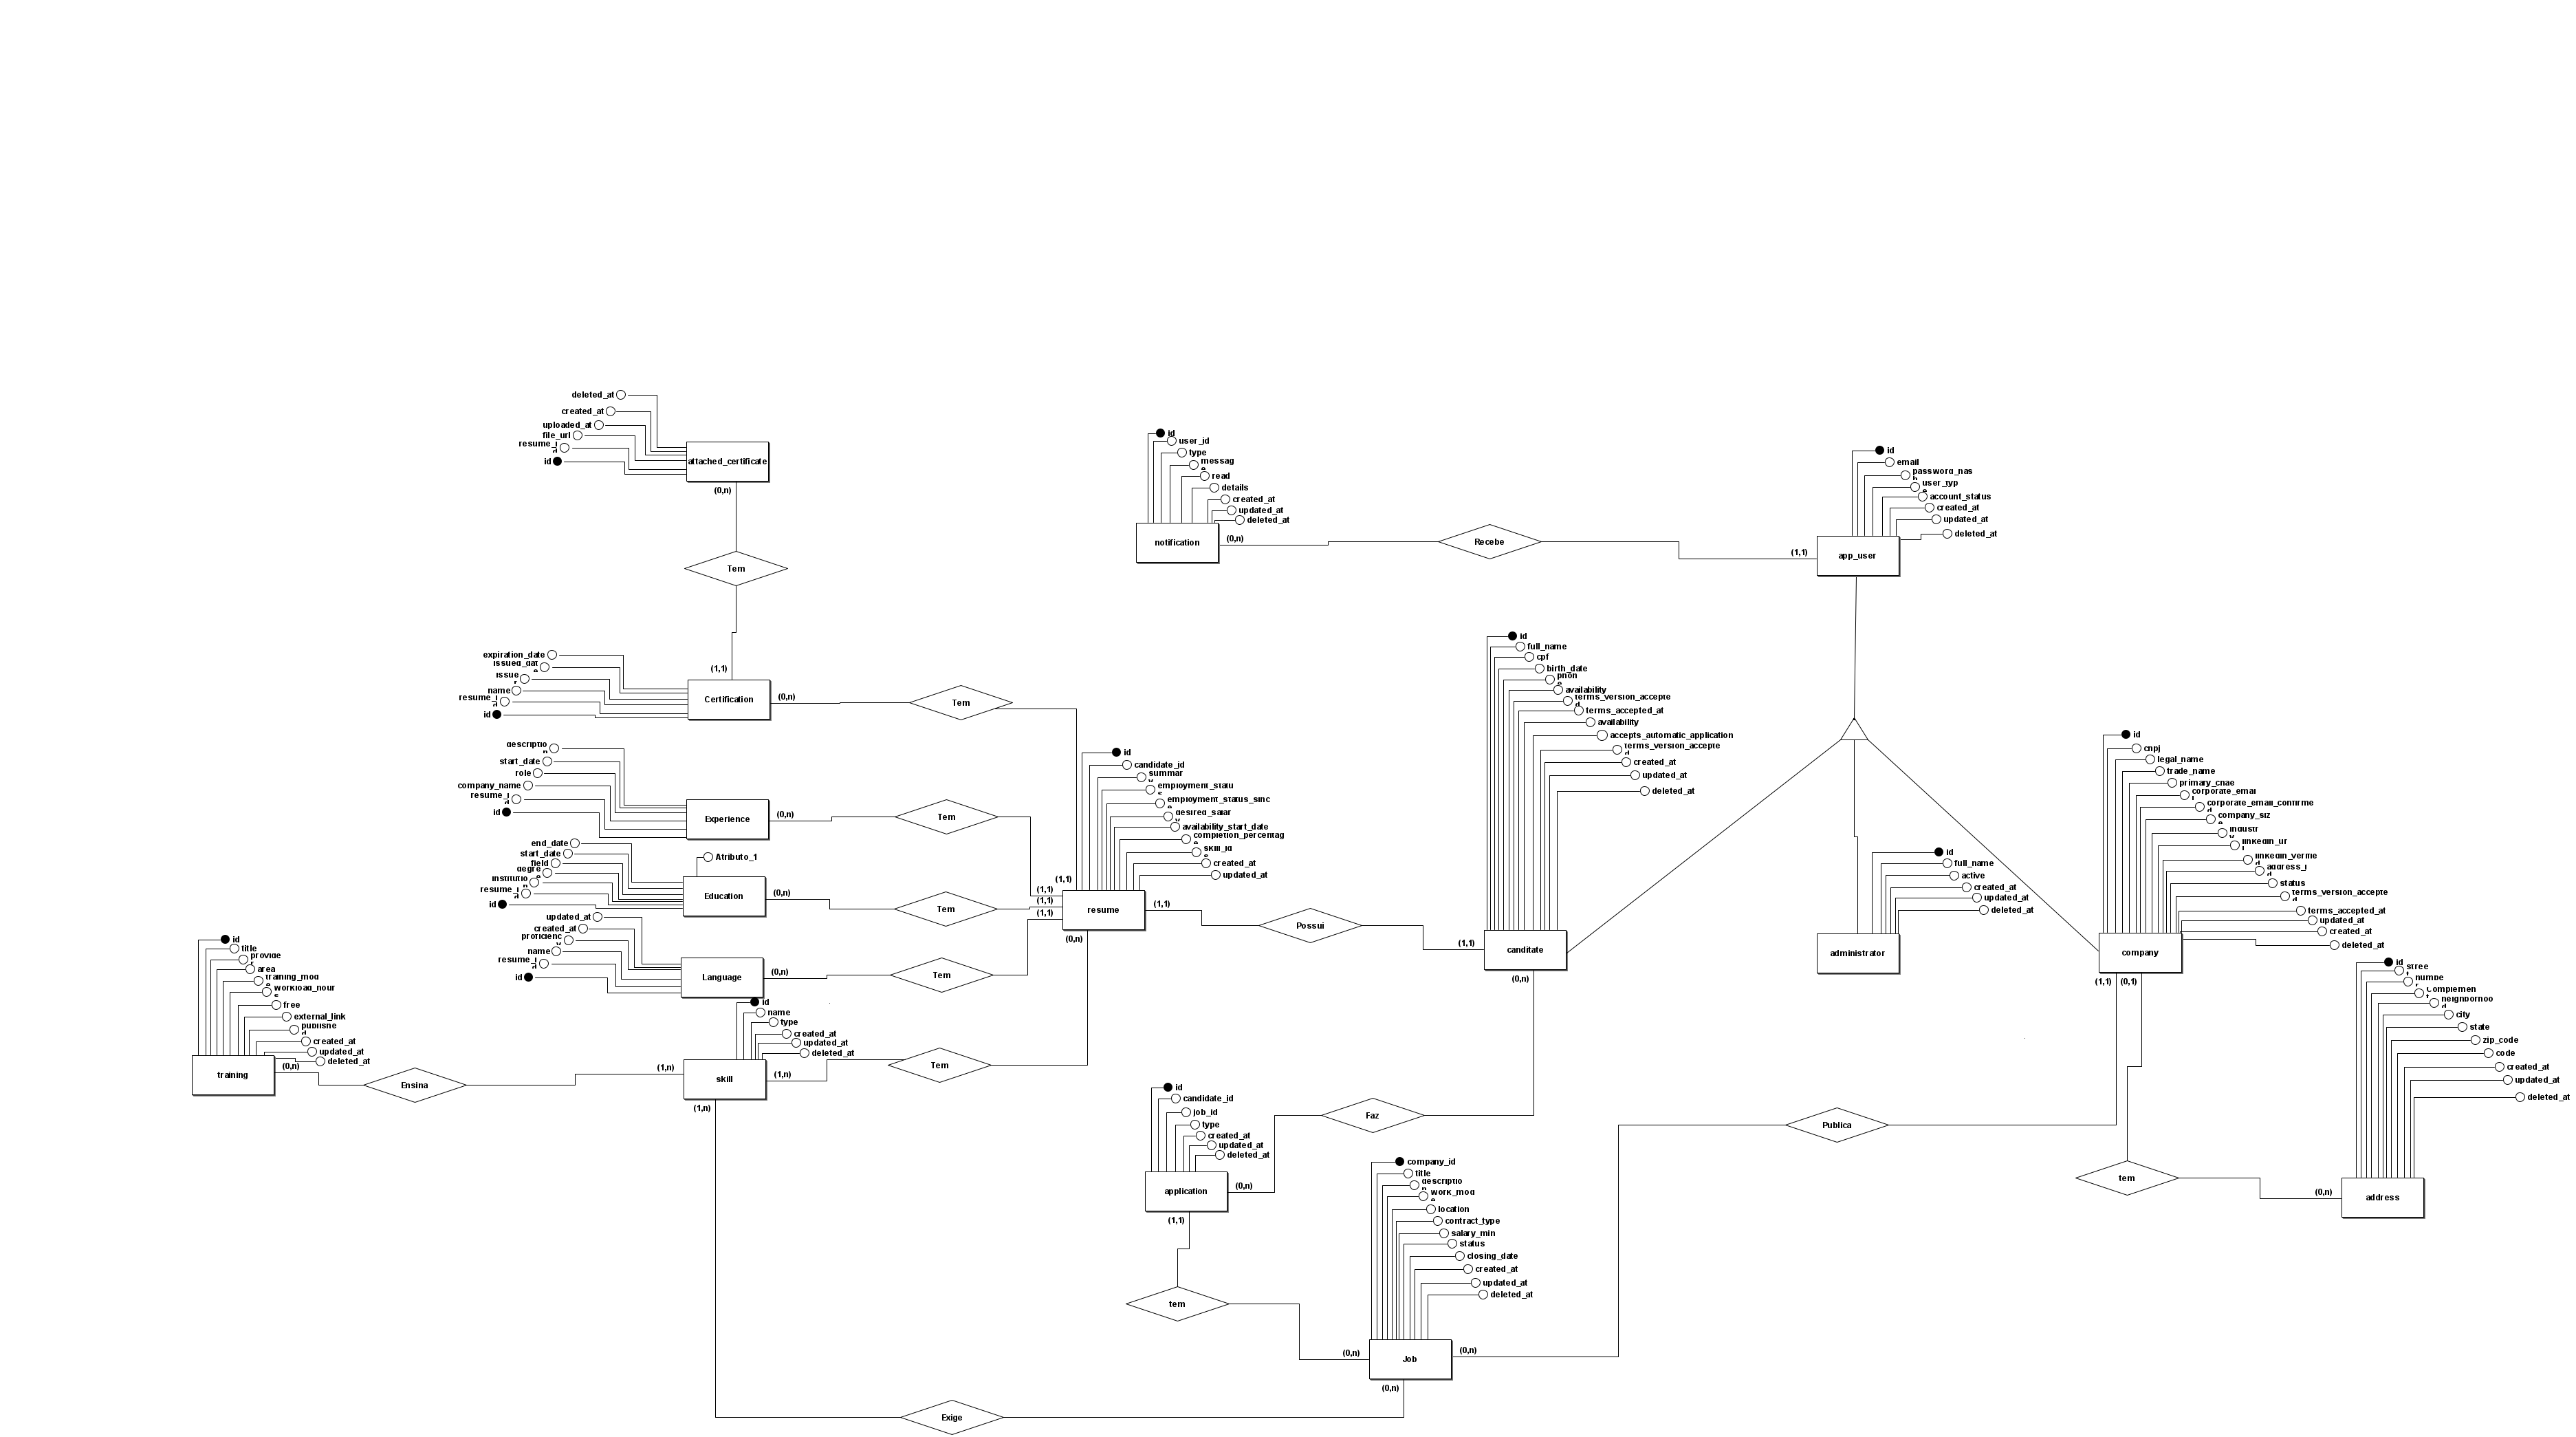
\includegraphics[width=1\linewidth]{conteudo/5 - ages IV/figures/senior_conceitual.png}
  Fonte: \textit{Wiki} do projeto
  \label{fig:db-concept-seniors}
\end{figure}

\begin{figure}[H]
  \centering
  \small
  \caption{Diagrama lógico do banco de dados do projeto Seniors -- Empregabilidade}
  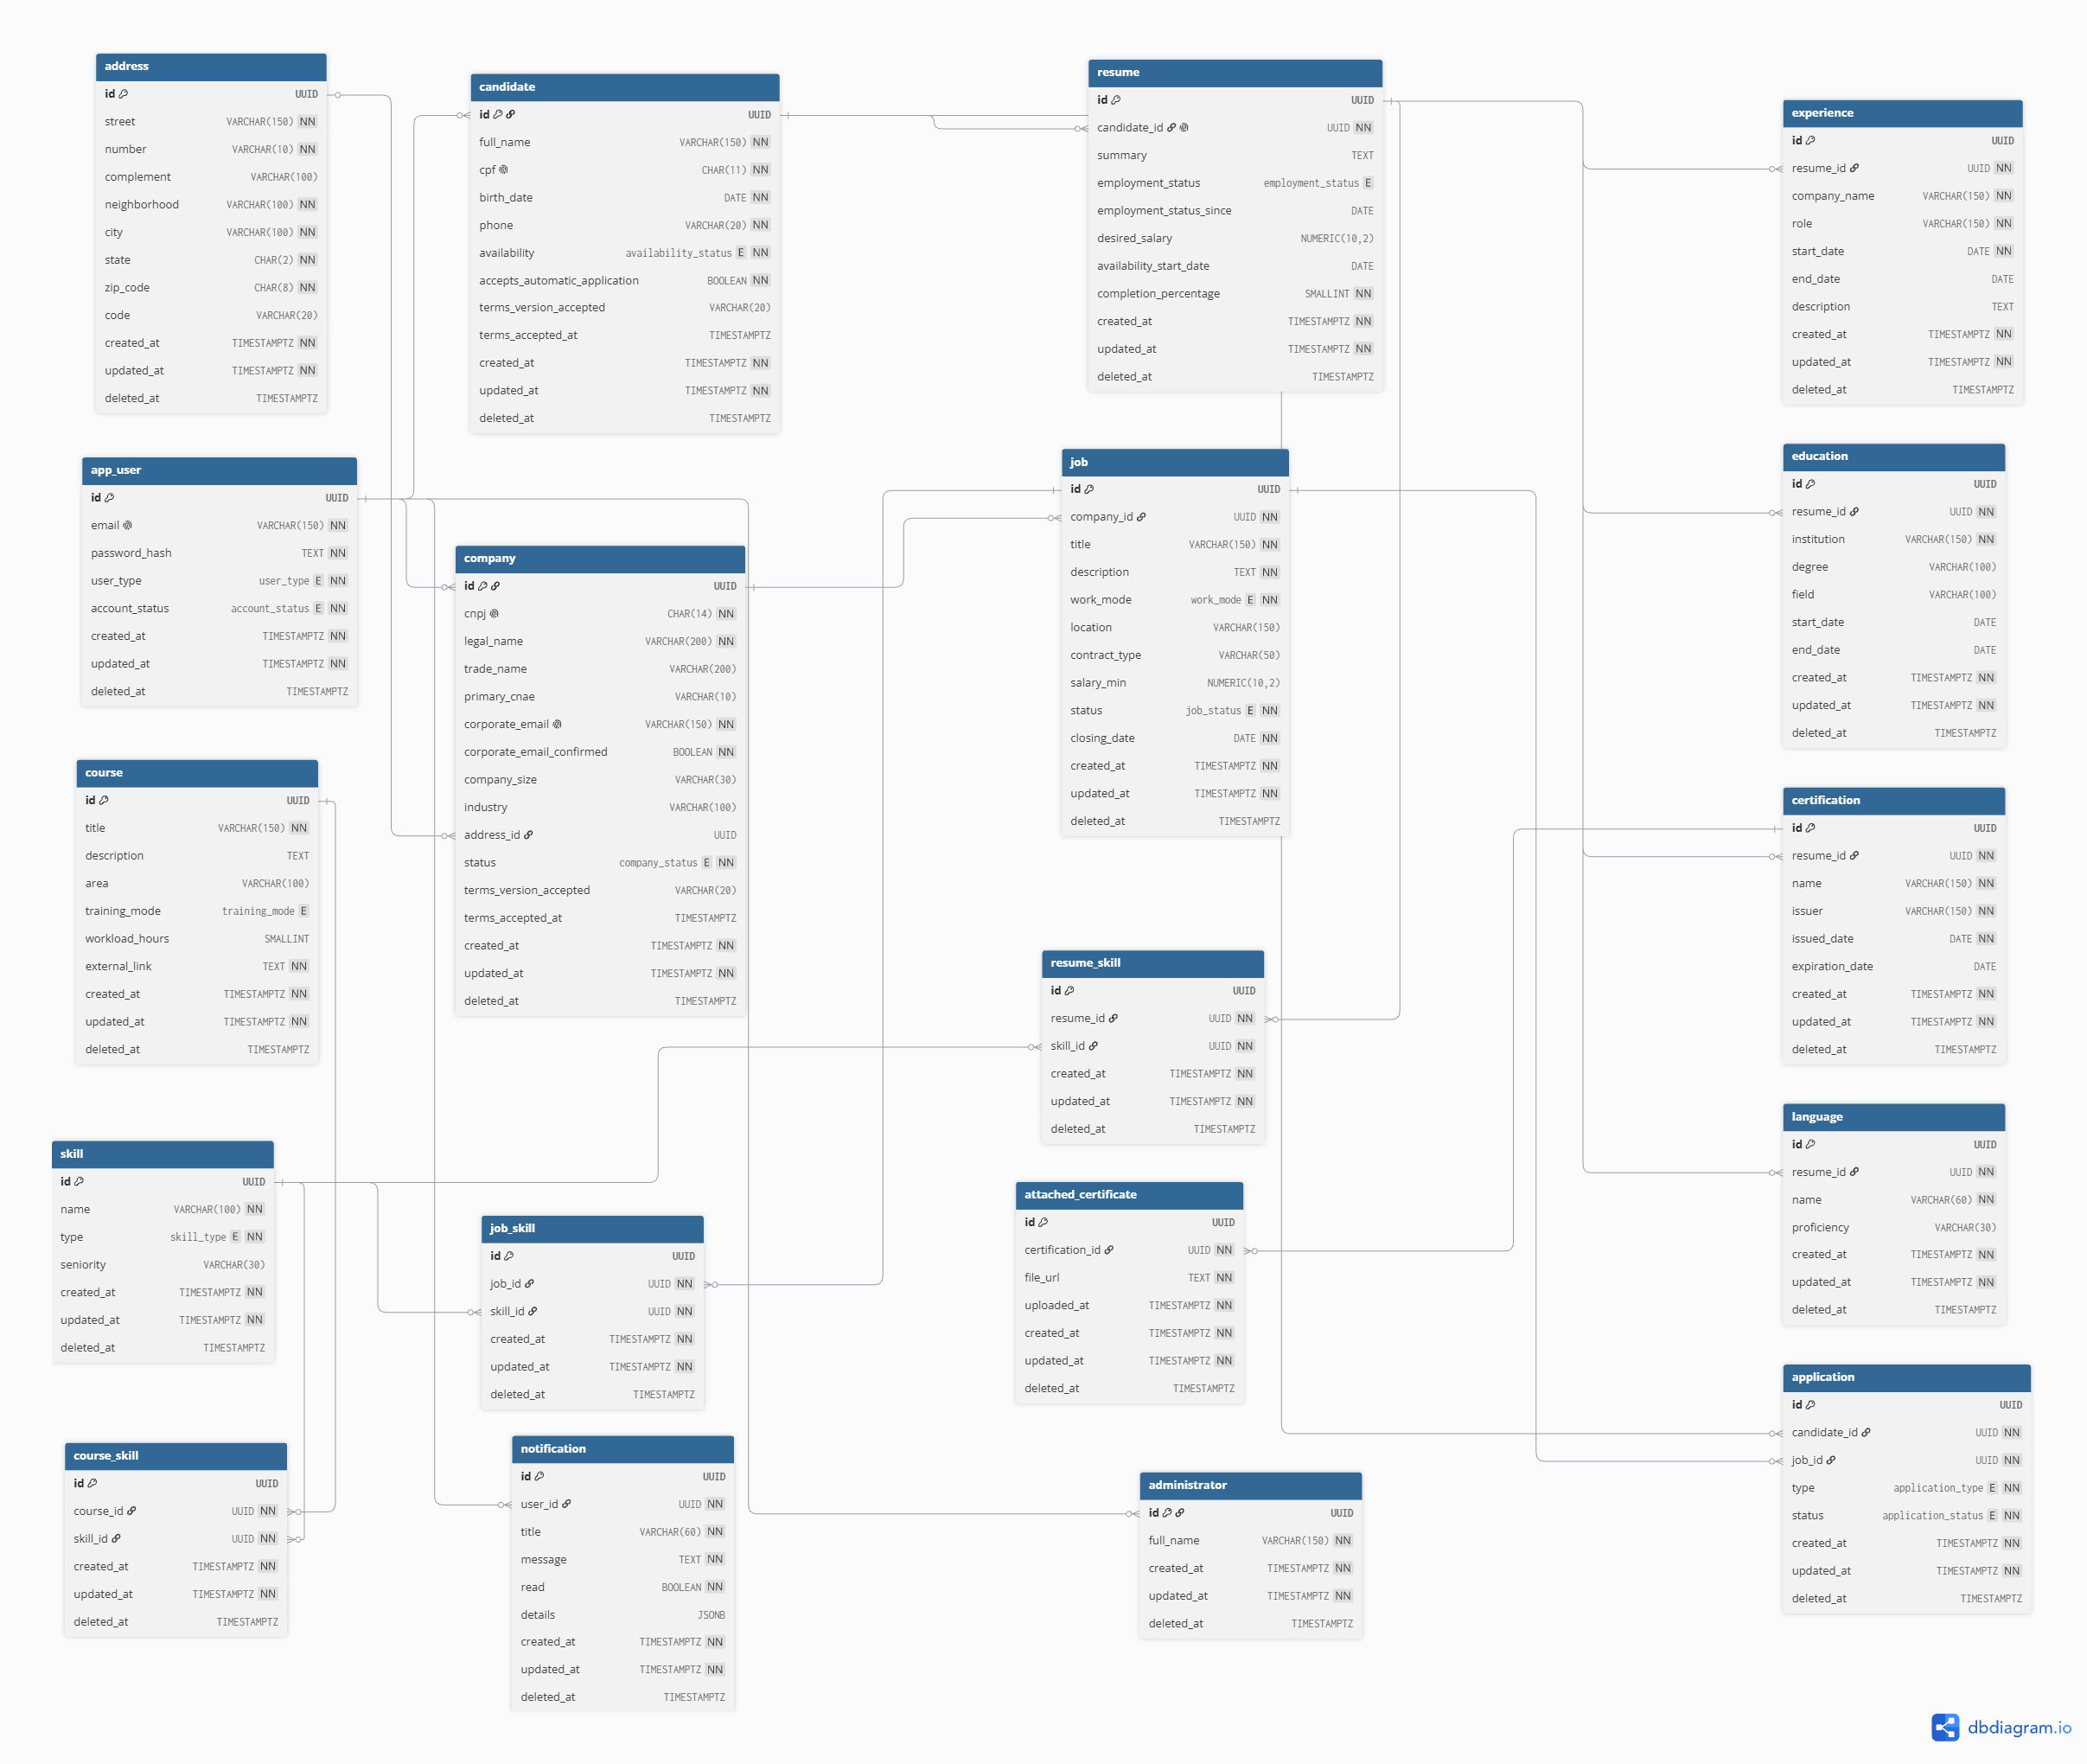
\includegraphics[width=1\linewidth]{conteudo/5 - ages IV/figures/senior_logical.png}
  Fonte: \textit{Wiki} do projeto
  \label{fig:db-logic-seniors}
\end{figure}

Entre as decisões de modelagem, destacam-se o uso de UUIDs como chaves primárias,
a separação dos perfis de candidato, empresa e administrador a partir de uma
entidade comum de usuário e o emprego de tabelas associativas para as relações
muitos-para-muitos entre currículos, vagas, cursos e habilidades. O modelo também
prevê restrições de integridade, como validações para CPF, CNPJ e idade mínima dos
candidatos, bem como a exclusão lógica dos registros para preservar o histórico.

A documentação detalhada, incluindo o dicionário de dados e as decisões de
modelagem, está disponível na \textit{Wiki} do projeto em:
\url{https://tools.ages.pucrs.br/2026-2/2lm-4lm/seniors-empregabilidade/seniors-empregabilidade-wiki/-/wikis/Banco%20de%20Dados}.

\subsection{Arquitetura Utilizada}
A arquitetura planejada para o projeto utiliza serviços da \ac{aws}, concentrados
na região \textit{us-east-1} e em uma única \ac{vpc}. A proposta prioriza serviços
gerenciados, mantendo em instância dedicada apenas a API da aplicação. Dessa forma,
a interface Web será hospedada no AWS Amplify e disponibilizada por meio do Amazon
Route 53, enquanto a autenticação dos usuários será centralizada no Amazon Cognito.
Essa estrutura é apresentada na Figura~\ref{fig:infra-seniors}.

\begin{figure}[H]
  \centering
  \small
  \caption{Diagrama da infraestrutura planejada do projeto Seniors -- Empregabilidade}
  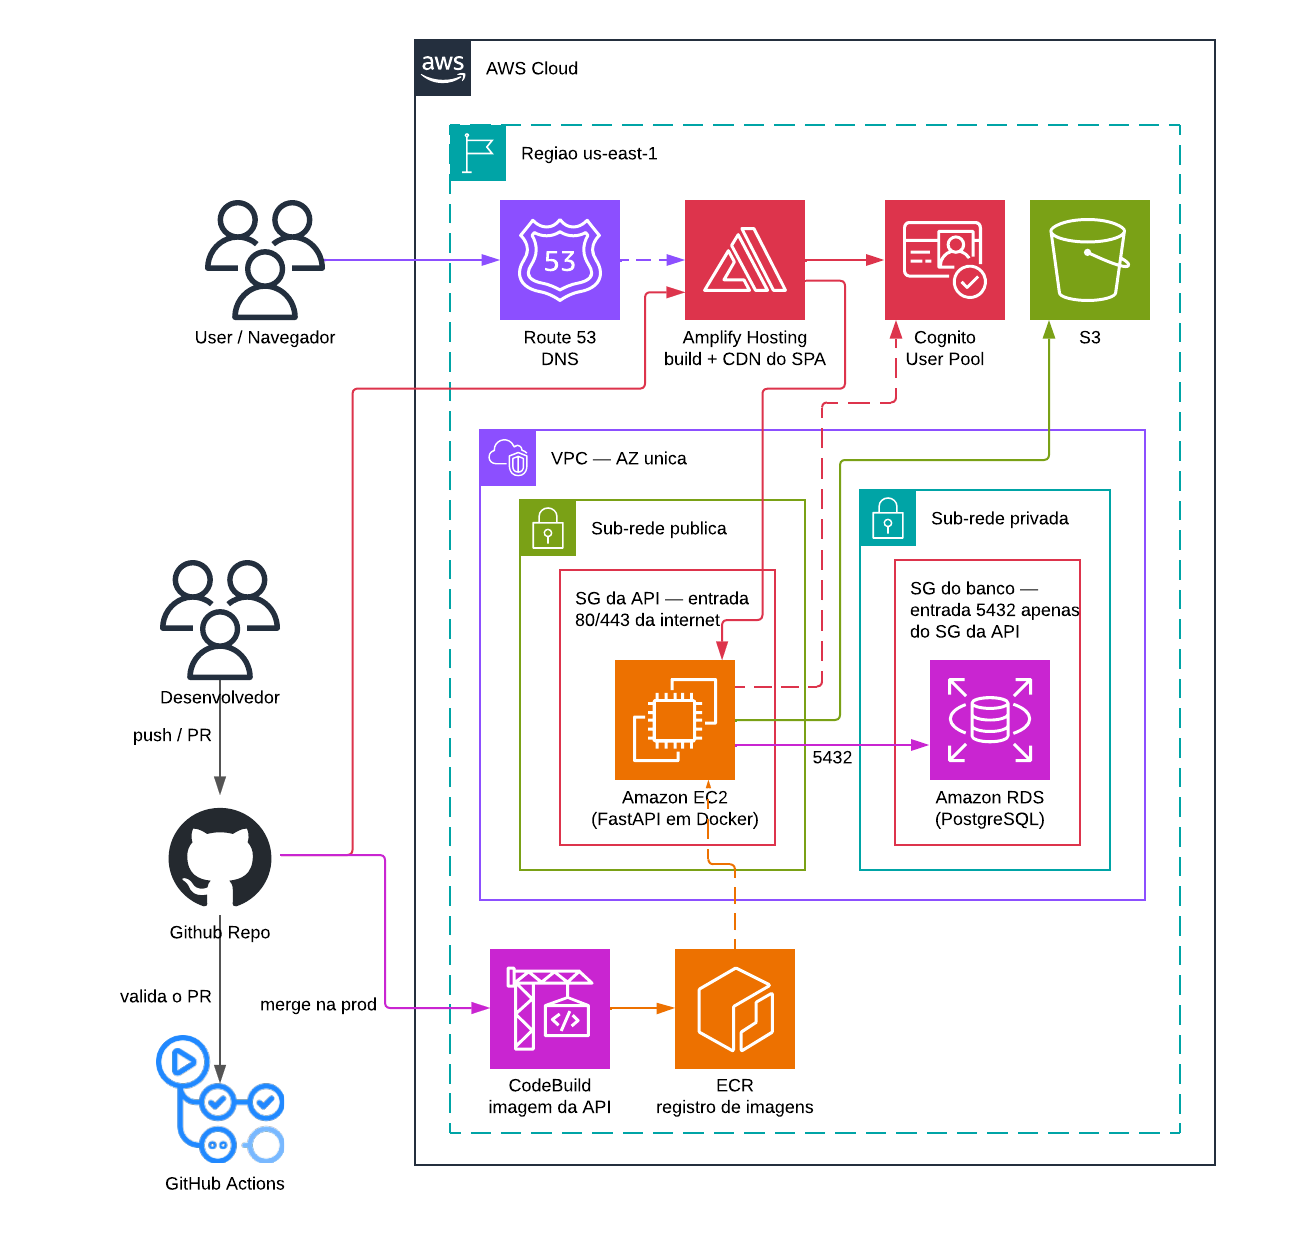
\includegraphics[width=1\linewidth]{conteudo/5 - ages IV/figures/Diagrama_de_Deploy_v2___Infraestrutura_AWS__pós-devolutiva_.png}
  Fonte: \textit{Wiki} do projeto
  \label{fig:infra-seniors}
\end{figure}

O \textit{backend} foi projetado para executar uma API FastAPI em um contêiner
Docker hospedado em uma instância \ac{ec2}, posicionada em uma sub-rede pública. A
API deverá validar os tokens emitidos pelo Cognito, comunicar-se com o banco
PostgreSQL hospedado no Amazon RDS, em sub-rede privada, e utilizar o Amazon S3
para o armazenamento de arquivos enviados pelos usuários, como currículos e
documentos. A separação entre as sub-redes e os grupos de segurança previstos
restringem o acesso ao banco de dados à própria API.

Também foi definido um fluxo de \ac{cicd} separado para os dois repositórios de
código. Os \textit{pull requests} serão validados pelo GitHub Actions. Após a
integração na \textit{branch} de produção, o AWS CodeBuild deverá construir a
imagem Docker da API, publicá-la no Amazon ECR e solicitar a atualização da
instância EC2. Em paralelo, o AWS Amplify realizará o \textit{build} e a
publicação do \textit{frontend}.

A documentação detalhada da infraestrutura planejada, incluindo o diagrama de
arquitetura, está disponível na \textit{Wiki} do projeto em:
\url{https://tools.ages.pucrs.br/2026-2/2lm-4lm/seniors-empregabilidade/seniors-empregabilidade-wiki/-/wikis/Infraestrutura}.

\subsection{Protótipos das Telas Desenvolvidas}
  Deverão ser apresentados os links da Wiki, com uma breve descrição.

\subsection{Tecnologias Utilizadas}
  Deverão ser apresentados os links da Wiki, com uma breve descrição.
  
  As tecnologias citadas deverão ter referências bibliográficas.
